\documentclass[a4paper,11pt]{article}
\usepackage[polish]{babel}
\usepackage[utf8]{inputenc}   % lub utf8
\usepackage[T1]{fontenc}
\usepackage{graphicx}
\usepackage{anysize}
\usepackage{enumerate}
\usepackage{times}
 
%\marginsize{left}{right}{top}{bottom}
\marginsize{3cm}{3cm}{3cm}{3cm}
\setlength{\parindent}{1em}
\sloppy


\title{Inżynieria Oprogramowania - analiza systemu aquaparku}
\date{2019/20}
\author{Piotr Wawrzynów \and Wojciech Dolata} 

\begin{document}
 
\maketitle
\newpage



\tableofcontents
\newpage


 
\section{Streszczenie systemu}
Modelowany przez nas system jest systemem obsługi aquaparku. System ten posiada obsługę zawierania transakcji kupna biletu jednorazowego, oraz karnetów okresowych zarówno na miejscu, jak i on-line. Klient po założeniu konta na stronie internetowej może za jej pomocą zakupić karnet, który jest na stałe przypisany do konta. Płatność internetowa odbywa się za pomocą pośrednika oferującego system takich płatności. Na miejscu istnieje możliwość płatności kartą lub gotówką. Jednym z zadań systemu jest również obsługa księgowości, czyli między innymi wystawianie faktur dla podwykonawców (np. firma ratownicza, firma sprzątająca), rozliczanie podatku VAT.\\ \\
System umożliwia również korzystanie z usług firmy gastronomicznej, której za pewną kwotę udostępnia się wydzielone miejsce na terenie aquaparku. Firma zapewniająca bezpieczeństwo w wodzie dostarcza wykwalifikowaną kadrę ratowniczą. W systemie instruktor prowadzi lekcje pływania dla dzieci i młodzieży oraz zajęcia aerobiku dla seniorów. Aquapark na potrzeby lekcji rezerwuje tor w basenie, na którym instruktor prowadzi zajęcia doskonalące technikę pływania, lub pojedynczy basen, w którym odbywają się zajęcia aerobiku.
\newpage


\section{Obiekty}
\begin{itemize}
    \item Klient - osoba korzystająca z usług aquaparku
    \item Pracownicy aquaparku
            \begin{itemize}
                \item Kasjer - osoba przyjmująca wpłaty i wydająca bilety wstępu
                \item Instruktor - nauczyciel pływania
                \item Księgowy - osoba zajmująca się szeroko pojętymi finansami
                \item Szatniarz - osoba odpowiedzialna za obsługę szatni
                \item Kierownik - osoba zatrudniająca firmy zewnętrzne
            \end{itemize}
    \item Narzędzia informatyczne
            \begin{itemize}
                \item strona internetowa - pozwala na otrzymanie informacji związanych z aquaparkiem oraz zakup biletu on-line
                \item program rozliczający - kalkuluje cenę biletu przy wstępie (system punktowy) lub przy wyjściu (system czasowy)
            \end{itemize}
    \item Firmy zewnętrzne
            \begin{itemize}
                \item firma sprzątająca
                \item firma obsługująca gastronomię
                \item firma obsługująca płatności internetowe (np. przelewy 24)
                \item firma ratownicza (np. WOPR)
            \end{itemize}
\end{itemize}



\section{Zdarzenia}
\begin{itemize}
    \item założenie konta stałego klienta
    \item zakup biletu jednorazowego lub karnetu
            \begin{itemize}
                \item on-line
                \item osobiście
            \end{itemize}
    \item rezerwacja toru (np. przez naukę pływania)
    \item wykupienie lekcji pływania
    \item uiszczenie płatności
    \item wybór sposobu płatności
            \begin{itemize}
                \item gotówka
                \item karta
            \end{itemize}
\end{itemize}
\newpage


\section{Diagram kontekstowy}
    \begin{figure}[!htb]
    \centerline{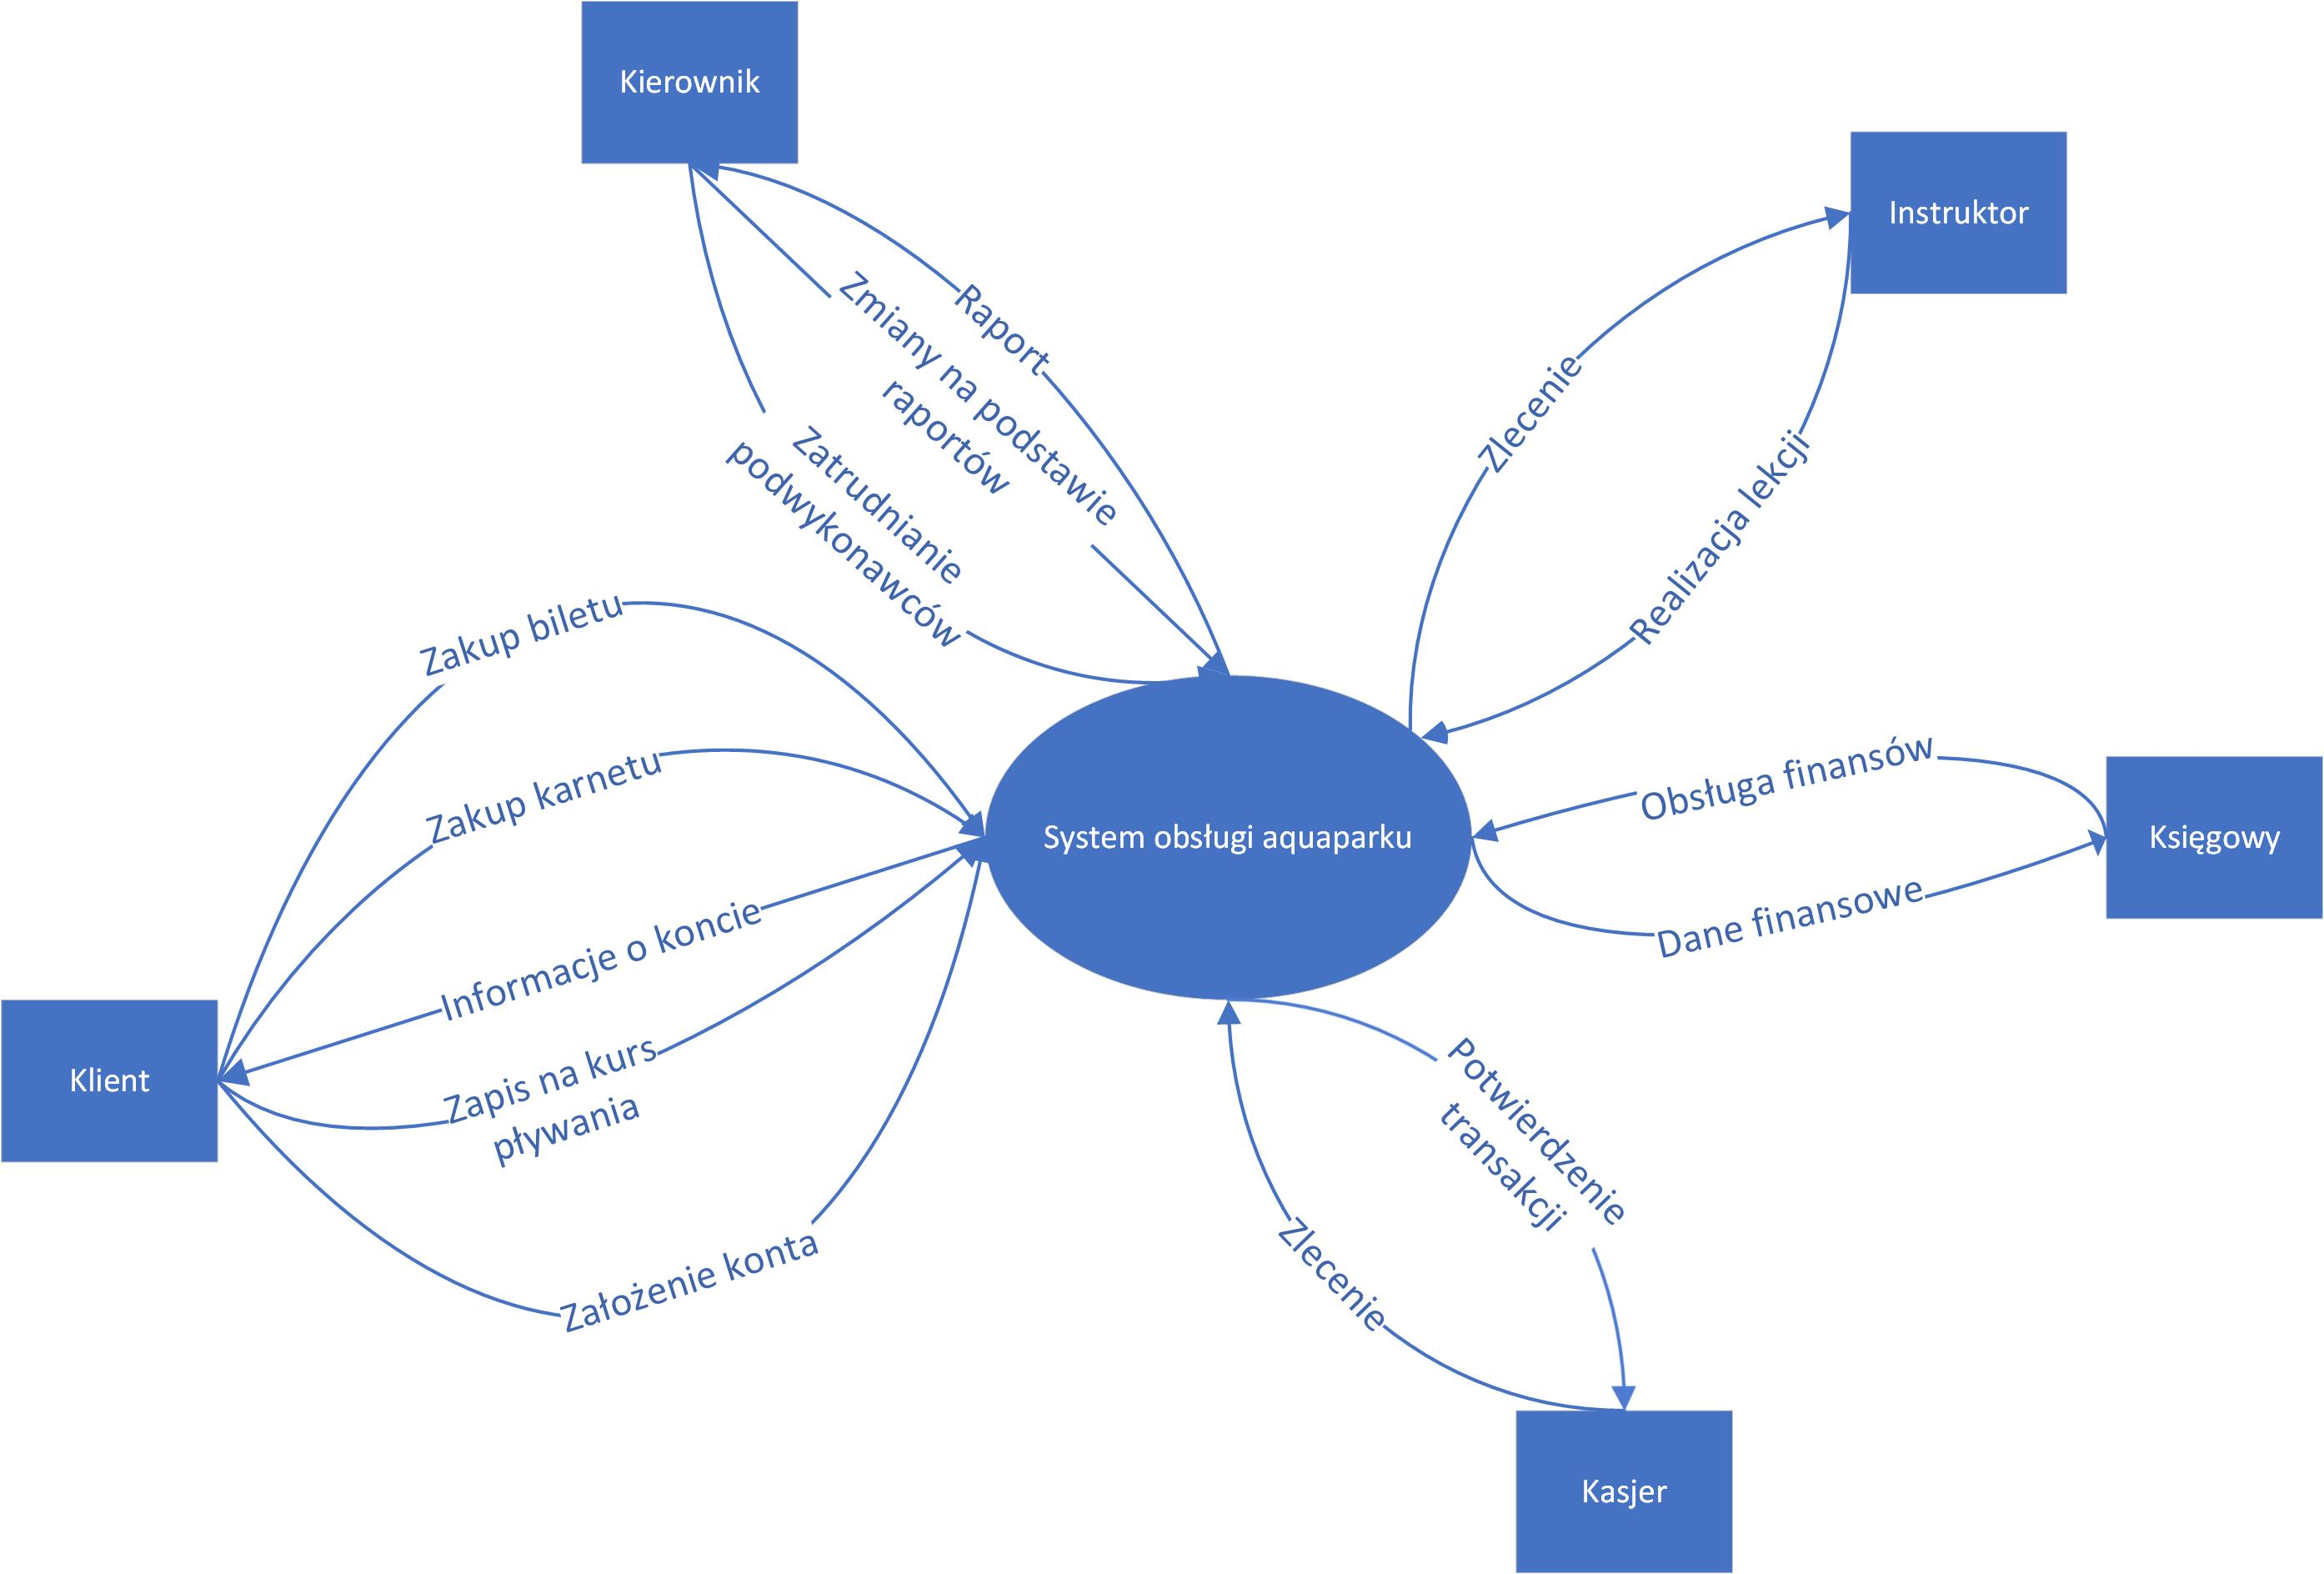
\includegraphics[scale=0.7]{kontekstowy.jpg}}
    \label{fig:kontekstowy}
    \end{figure}
\newpage



\section{Diagramy DFD}
\subsection{Poziom 0}
    \begin{figure}[!htb]
    \centerline{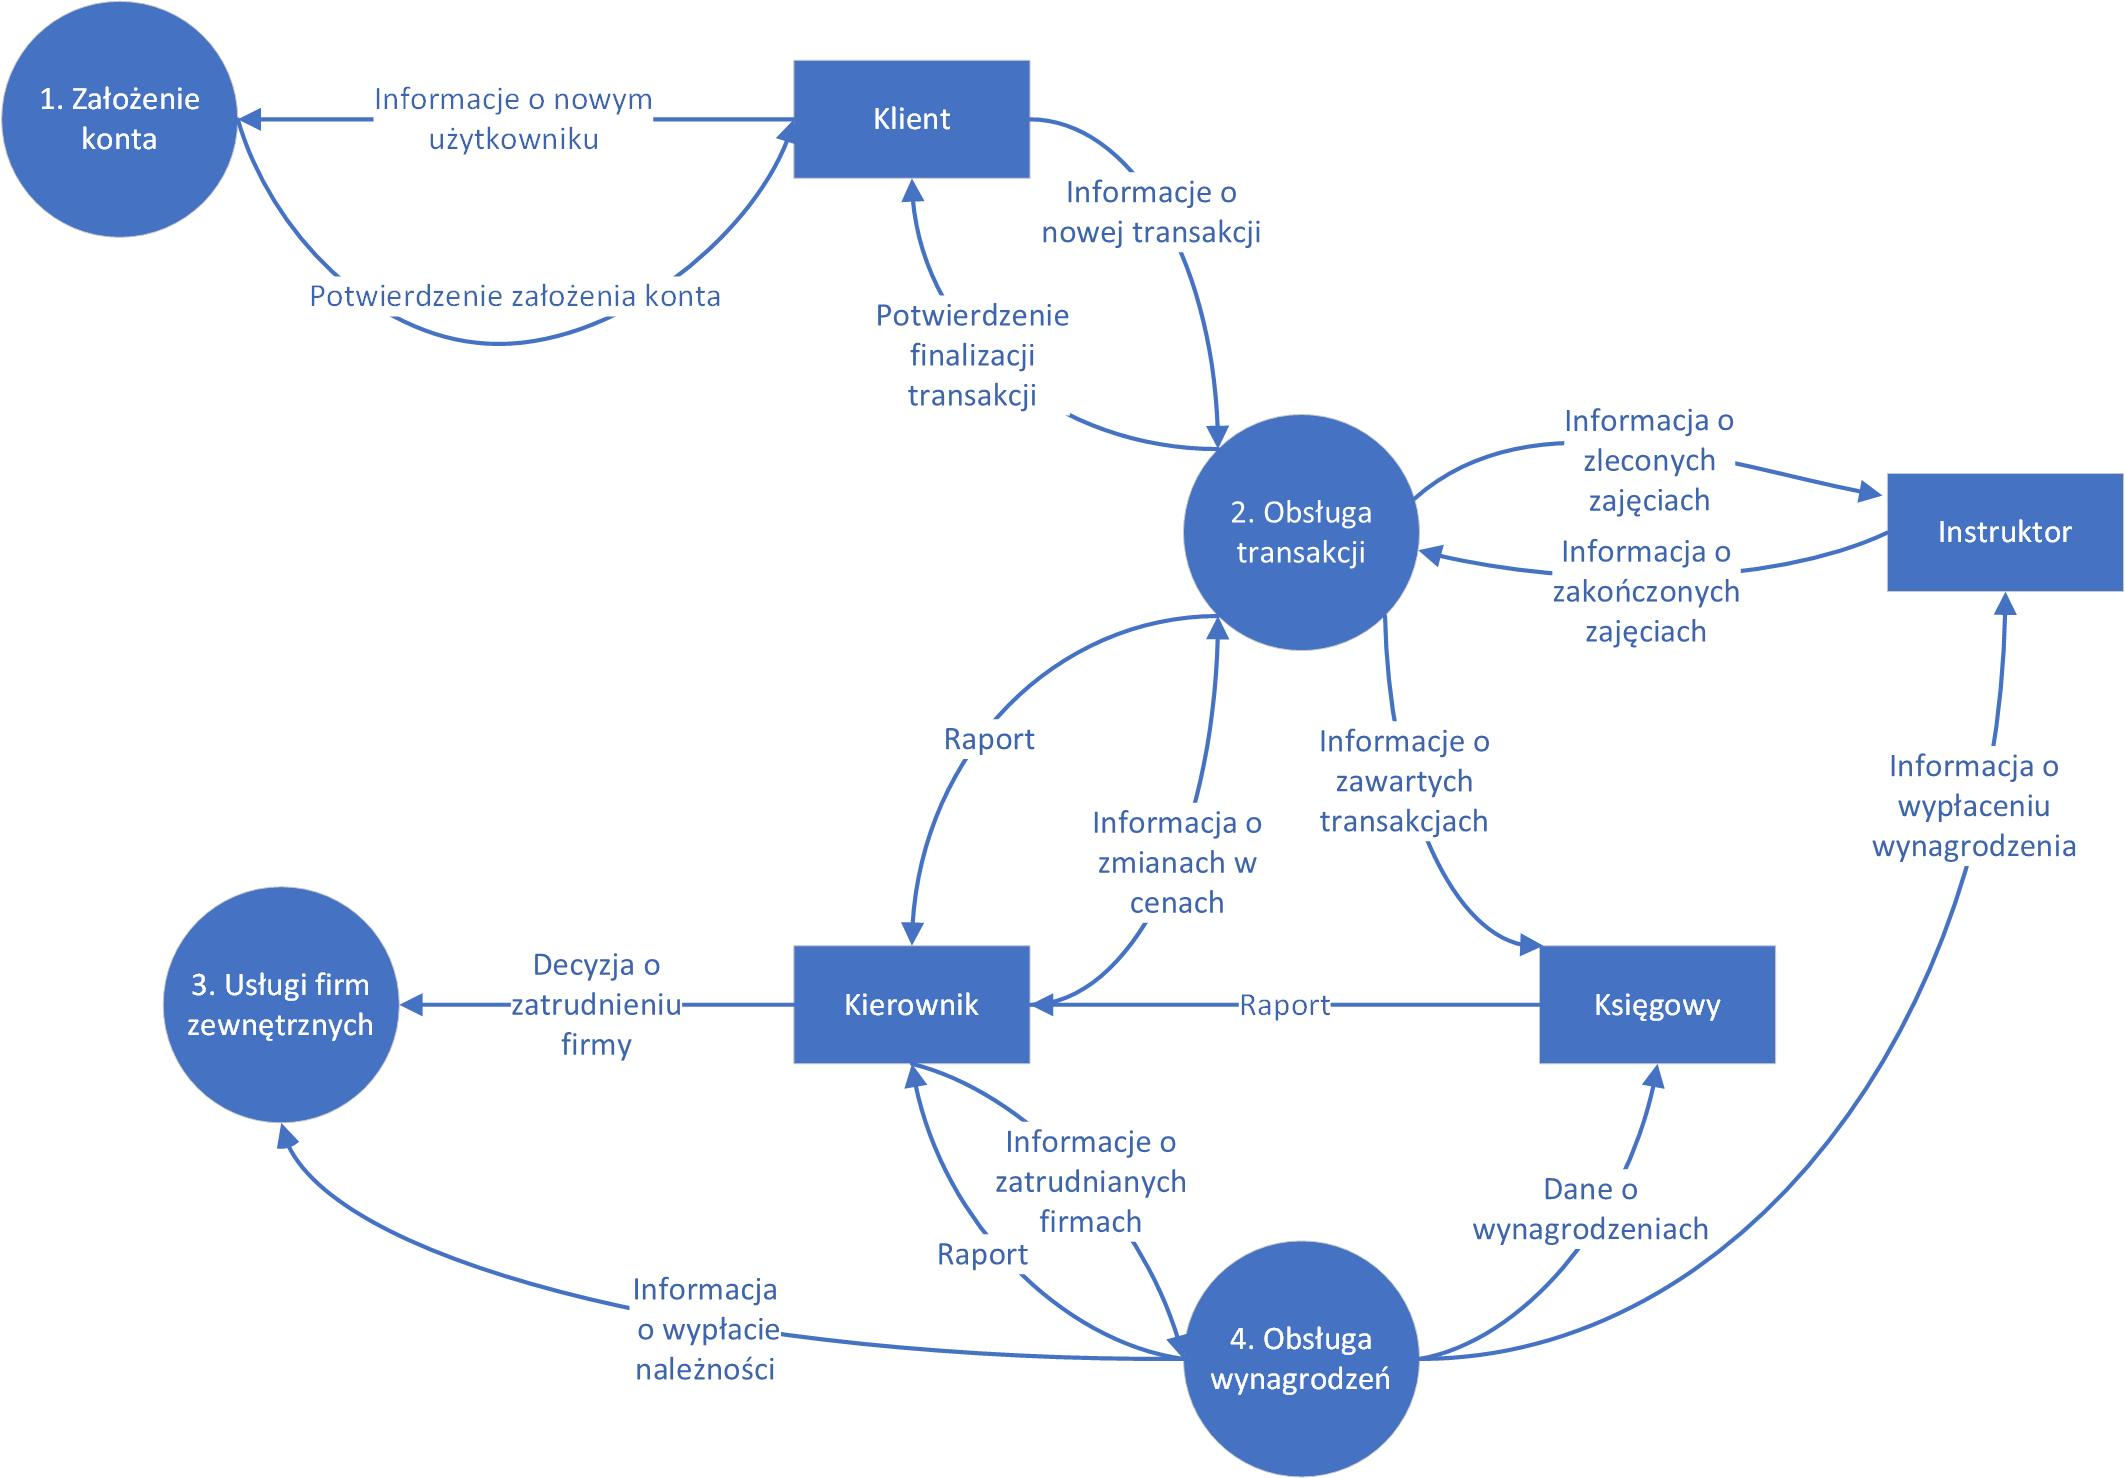
\includegraphics[scale=0.9]{level0.jpg}}
    \label{fig:level0}
    \end{figure}
\newpage



\subsection{Poziom 1}
\subsubsection{Dekompozycja procesu Założenie konta}
    \begin{figure}[!htb]
    \centerline{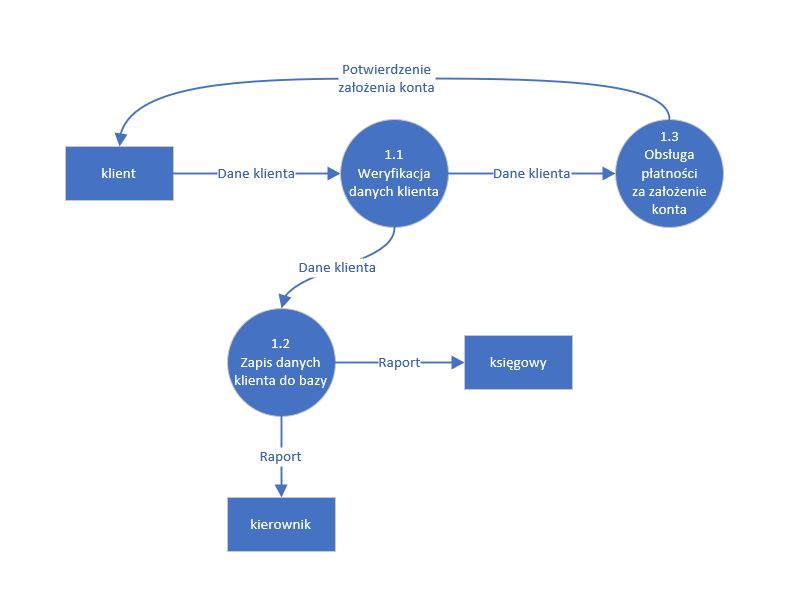
\includegraphics[scale=1.2]{level1_1.jpg}}
    \label{fig:level1_1}
    \end{figure}
    \newpage



\subsubsection{Dekompozycja procesu Obsługa transakcji}
    \begin{figure}[!htb]
    \centerline{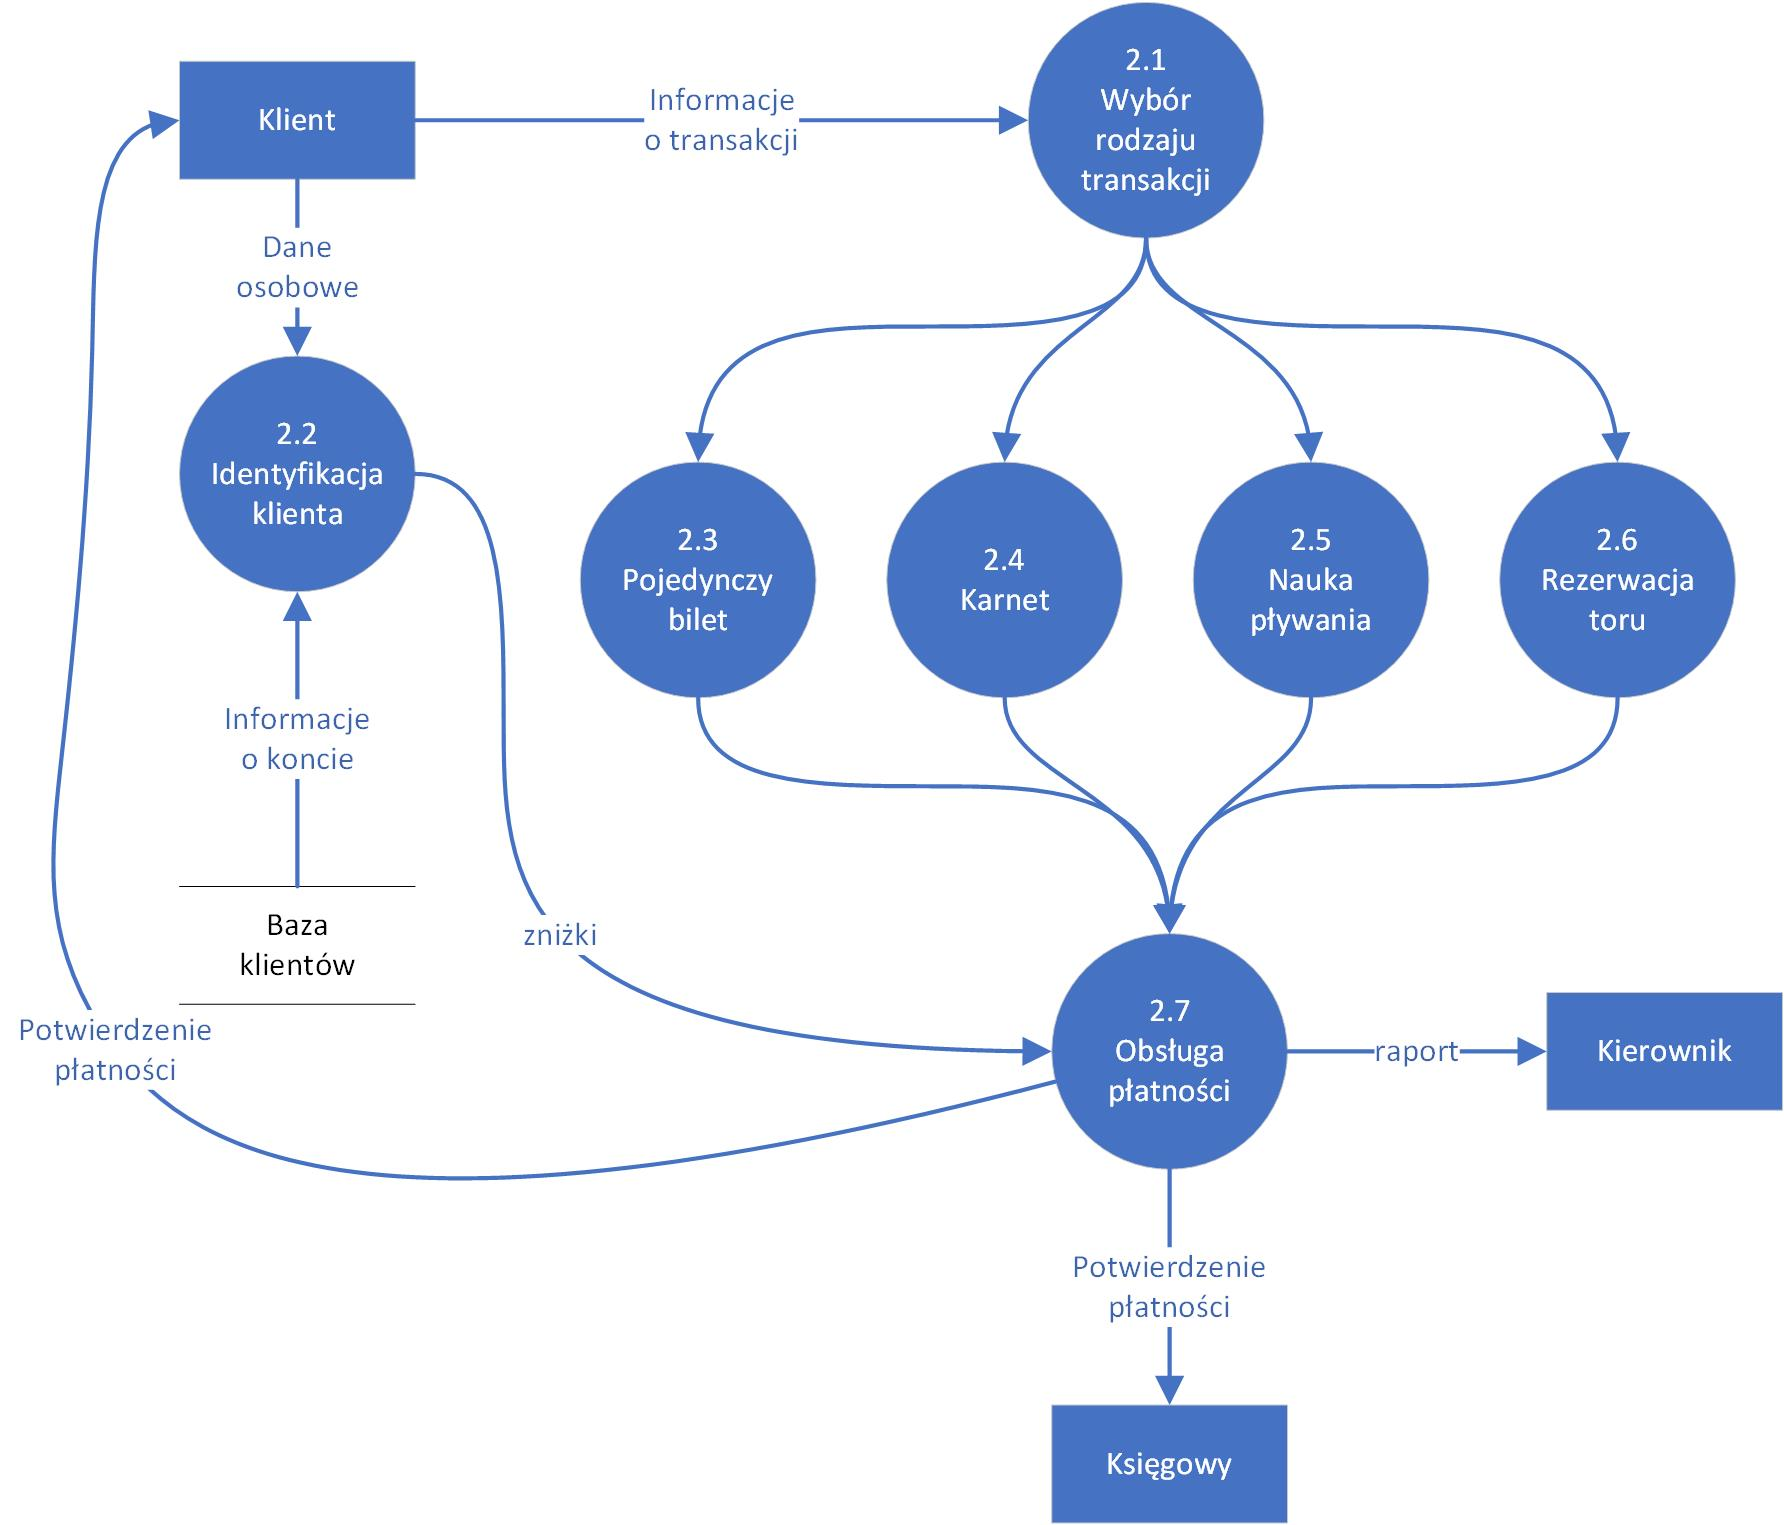
\includegraphics[scale=1.1]{level2_1.jpg}}
    \label{fig:level1_2}
    \end{figure}
    \newpage



\subsubsection{Dekompozycja procesu Usługi firm zewnętrznych}
    \begin{figure}[!htb]
    \centerline{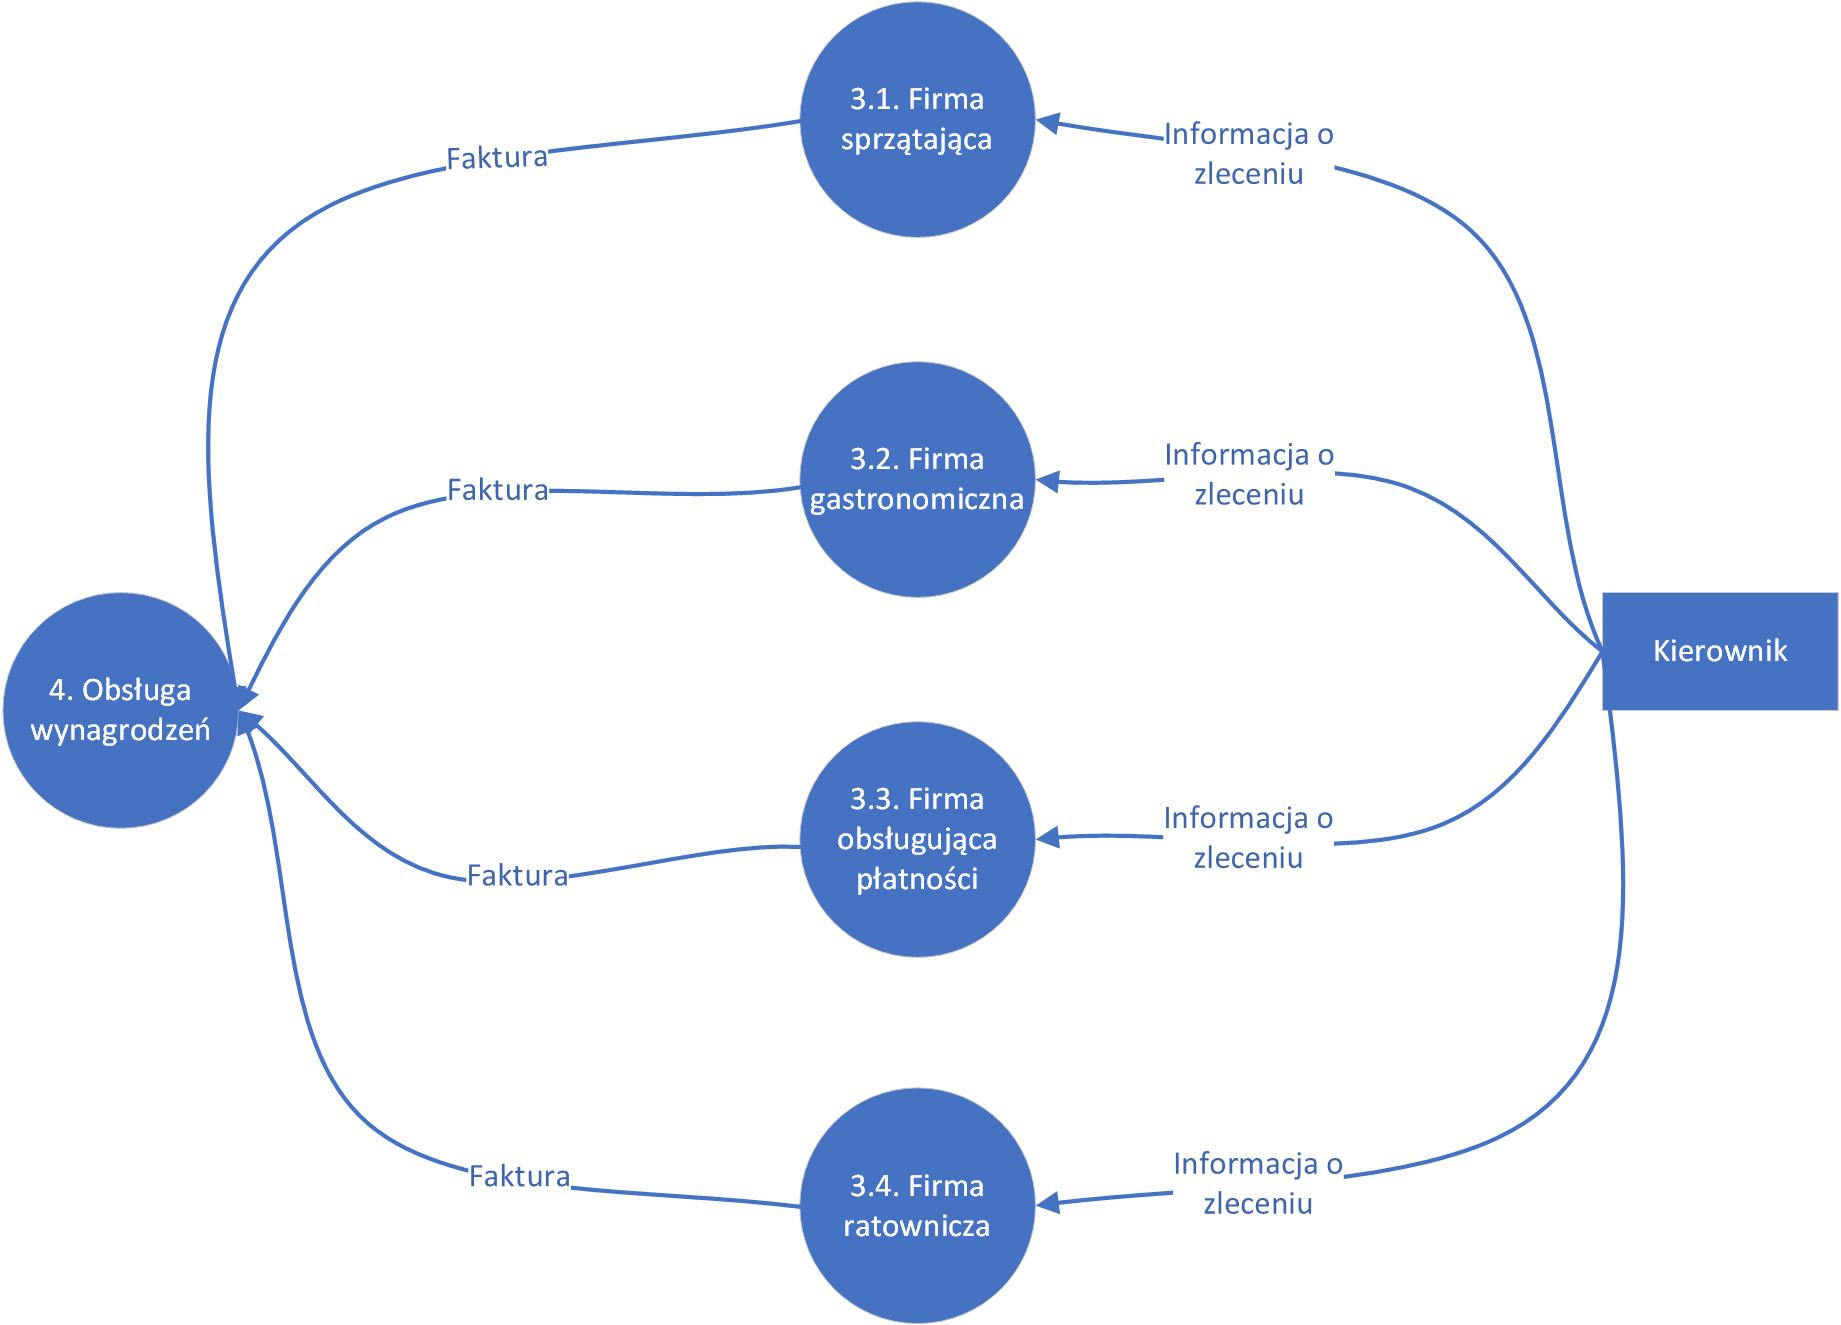
\includegraphics[scale=1.1]{level1_3.jpg}}
    \label{fig:level1_3}
    \end{figure}
    \newpage
    
    
    
    
\subsection{Poziom 2}
\newpage
 
\end{document}